\chapter{Kraftwirkung auf Ladungen und Ströme}

Erinnerung: \textbf{Lorentzkraftdichte}

\begin{equation*}
\vec{f}_L \ = \ \rho \ \vec{E} \ + \ \vec{j}\times\vec{B}
\end{equation*}

\section{Elektrischer Dipol}
\begin{wrapfigure}[12]{l}[0cm]{0cm}
	\raisebox{0pt}[\dimexpr\height-1\baselineskip\relax]{
		\colorbox{hgrey}{
			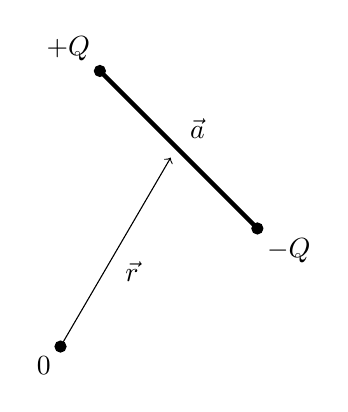
\begin{tikzpicture}
			
	\draw[ultra thick] (-1,1)--node[above right]{$\vec{a}$}(1,-1);
	\filldraw[black] (-1,1) circle (2pt) node[above left]{$+Q$};
	\filldraw[black] (1,-1) circle (2pt) node[below right]{$-Q$};
	\filldraw[black] (-1.5,-2.5) circle (2pt) node[below left]{$0$};
	\draw[->] (-1.5,-2.5) -- node[below right]{$\vec{r}$} (-0.1,-0.1);
			
			
			\end{tikzpicture}
		}
	}
	\caption{elektrischer Dipol}
\end{wrapfigure}
Wir betrachten einen elektrischen Dipol am Ort $\vec{r}$, dessen Ladungen den Abstand $\vec{a}$ voneinander haben. Die Kraft auf ihn beträgt:

\begin{equation*}
\vec{F} \ = \ Q \cdot \vec{E}\left(\vec{r} \ + \ \frac{\vec{a}}{2}\right) \ - \ Q \cdot\vec{E} \left(\vec{r} \ - \ \frac{\vec{a}}{2}\right) \qquad (=0 \text{ für $\vec{E}$ homogen})
\end{equation*}

Wir entwickeln diesen Ausdruck für das Dipollimit $|\vec{a}| \rightarrow 0$:

\begin{align*}
\vec{F}  \ &= \ Q \cdot \left( \vec{E} (\vec{r}) \ + \ \frac{1}{2} \left(\vec{a}\cdot\pdiff{}{\vec{r}}\right) \vec{E}(\vec{r}) \ - \ \vec{E}(\vec{r}) \ + \ \frac{1}{2} \left(\vec{a}\cdot\pdiff{}{\vec{r}}\right)\vec{E}(\vec{r})\right) \\
\vec{F} \ &= \ Q\cdot \left(\vec{a}\cdot\nabla\right) \ \vec{E}  \ = \ \left( \vec{p} \cdot \nabla\right) \ \vec{E}
\end{align*}

Den Ausdruck für das Drehmoment auf einen Dipol im elektrischen Feld erhalten wir analog:

\begin{align*}
\vec{M}  \ &= \ Q \cdot \left(\frac{\vec{a}}{2} \times \vec{E}\left(\vec{r} \ + \ \frac{a}{2}\right) \ + \ \frac{\vec{a}}{2} \times \vec{E}\left(\vec{r} \ - \ \frac{\vec{a}}{2}\right)\right)\\
\vec{M}  \ &= \ Q \cdot \vec{a}\times\vec{E}  \ = \ \vec{p}\times\vec{E} 
\end{align*}

\section{Magnetischer Dipol}
\begin{wrapfigure}[10]{l}[0cm]{0cm}
	\raisebox{0pt}[\dimexpr\height-1\baselineskip\relax]{
		\colorbox{hgrey}{
			\begin{tikzpicture}
			
				\draw[ultra thick, -latex] (0,0) [partial ellipse=40:410:2cm and 0.5cm];
				\draw (1.6,0.4) node[above right]{$I$};
				\filldraw[black] (-1.5,-2.5) circle (2pt) node[below left]{$0$};
				\draw[->] (-1.5,-2.5) -- node[below right]{$\vec{r}$} (0,0);
				\draw[->] (-1.5,-2.5) -- node[left]{$\vec{r}'$} (-2,-0.2);
				\draw[->] (-0.1,0) -- node[above]{$\ \ \vec{r}''$} (-1.8,0);
			
			
			\end{tikzpicture}
		}
	}
	\caption{magnetischer Dipol}
\end{wrapfigure}
Wir betrachten einen Kreisstrom $I$, dessen Mittelpunkt sich am Ort $\vec{r}$ befindet und welcher die Fläche $\vec{A}_F$ umschließt und somit ein Dipolmoment von $\vec{m} = I \cdot \vec{A}_F$ erzeugt. Die Kraft auf diesen magnetischen Dipol beträgt: ($\vec{r}'$ ist dabei ein Ort auf dem Rand des Kreisstroms)

\begin{align*}
\vec{F} \ &= \ \Int{}{}{V'} \ \vec{j}(\vec{r}') \times \vec{B}  \ = \ I \ \Oint{}{}{\vec{r}'} \times\vec{B} \qquad \\
&(= 0 \text{ für homogenes Feld})\\
\vec{F} \ &= \ I \ \Oint{}{}{\vec{r}'} \times \vec{B}(\vec{r'} - \ \vec{r}'') \qquad \text{mit }\  \vec{r}''  = \ \vec{r}' - \ \vec{r} 
\end{align*}

Wir entwickeln für $|\vec{r}''| \ll |\vec{r}|$: 

\begin{align*}
\vec{F} \ &= \ I \ \Oint{}{}{\vec{r}'} \times \Bigg[ \underbrace{\vec{B}(\vec{r})}_{=0} \ + \ \left(\vec{r}'' \cdot\pdiff{}{\vec{r}}\right)\vec{B}(\vec{r})\Bigg]\\
&= \ I \ \underbrace{\Oint{}{}{\vec{r}'}\times\left(\vec{r}'' \cdot \pdiff{}{\vec{r}}\right)}_{(*)}\vec{B}(\vec{r}) 
\end{align*}

Lösung des Integrals $(*)$:

\begin{align*}
\Oint{}{}{\vec{r}'} (\vec{r}''\cdot \ \vec{a}) & \quad = \quad \ \oint{}{}{\vec{r}'} \cdot (\vec{r'}- \ \underbrace{\vec{r}}_{=0}) \vec{a}\\
& \overset{\text{Kap. 5.3}}{=} \ \frac{1}{2}\oint(\vec{r}'\times\d\vec{r}')\times\vec{a} \ + \ \frac{1}{2}\Oint{}{}{\vec{r}'}(\vec{r}'\cdot\vec{a})\\
& \quad = \quad \ \vec{A}_F \times\vec{a}
\end{align*}

$\Rightarrow\quad$ Einsetzen:

\begin{align*}
\vec{F}  \ &= \ \underbrace{I \ (\vec{A}_F}_{\vec{m}} \times \nabla)\times \vec{B} \ \overset{\text{bac-cab}}{=} \ \nabla(\vec{m}\cdot\overset{\downarrow}{\vec{B}}) \ - \ \vec{m}(\underbrace{\nabla\cdot\overset{\downarrow}{\vec{B}}}_{=0})\\
\vec{F}  \ &= \ \nabla(\vec{m}\cdot\vec{B}) \ \overset{\text{bac-cab}}{=} \ \vec{m} \times (\underbrace{\nabla\times\vec{B}}_{(**)}) \ + \ (\vec{m}\cdot\nabla)\vec{B}
\end{align*}

$(**)=0$, da $\dot{\vec{E}}=0$ und $\mu_0\vec{j}\rightarrow 0$ außerhalb der Quellen.\\
Somit :

\begin{equation*}
\vec{F}  \ = \  (\vec{m}\cdot\nabla) \vec{B} \qquad\qquad (\text{vgl. el. Dipol: } \vec{F}  \ = \ (\vec{p}\cdot\nabla)\vec{E})
\end{equation*}

Für das Drehmoment auf den magnetischen Dipol gilt:

\begin{align*}
\vec{M}  \ &= \ \Int{}{}{V'} \vec{r}\times\left[\vec{j}(\vec{r}') \times \vec{B}(\vec{r}')\right] \ = \  I  \ \Oint{}{}{\vec{r}''} \times \left[\d\vec{r}' \times\vec{B}(\vec{r}')\right]\\
 &= \ I \ \Oint{}{}{\vec{r}'}(\vec{r}''\cdot\vec{B}(\vec{r}')) \ - \ I \ \oint(\d\vec{r}'\cdot\vec{r}'')\vec{B}(\vec{r}')
\end{align*}

Näherung: $\vec{B}$ ist homogen. Auflösung der Integrale:

\begin{align*}
&\Oint{}{}{\vec{r}'} \cdot \vec{r}'' \ = \ \Oint{}{}{\vec{r}'}\cdot\vec{r}'  \ = \ \oint\frac{1}{2}\d(\vec{r}'^2)  \ = \ 0\\
&\Oint{}{}{\vec{r}'} (\vec{r}''\cdot\ \vec{B})  \ = \ \vec{A}_F \times\vec{B} \qquad \text{wie in } (*)
\end{align*}

\begin{equation*}
\Rightarrow \quad \vec{M}  \ = \ I\cdot \vec{A}_F \times \vec{B} \ = \ \vec{m}\times\vec{B} \qquad\qquad (\text{vgl. el. Dipol: } \vec{M}  \ = \ \vec{p}\times\vec{E})
\end{equation*}

\section{Multipolentwicklung der elektrischen Wechselwirkungsenergie}

Wir betrachten zwei Ladungsverteilungen mit den Dichten $\rho_1$ und $\rho_2$, welche sich im Abstand $l$ voneinander befinden. Die gemeinsame elektrische Feldenergie beträgt:

\begin{equation*}
W_e \ = \ \frac{1}{8\pi\epsilon_0}\int\d V \d V' \frac{\left(\rho_1(\vec{r}) \ + \ \rho
_2(\vec{r})\right)\left(\rho_1 (\vec{r}') \ + \ \rho_2(\vec{r}')\right)}{|\vec{r} \ - \ \vec{r}'|}
\end{equation*}

Betrachten wir nun die Wechselwirkungsenergie zwischen 1 und 2, wozu wir annehmen, dass $\rho_1$ ein "äußeres" Potential $\varphi_1$ erzeugt, welches mit $\rho_2$ wechselwirkt:

\begin{equation*}
W_{12} \ = \  \frac{1}{4\pi\epsilon_0} \ \int\d V \d V' \ \frac{\rho_1(\vec{r})\rho_2(\vec{r}')}{|\vec{r}-\vec{r}'|} \ = \ \Int{}{}{V} \rho_2\varphi_1
\end{equation*}

Wir benennen nun der Einfachheit halber $\varphi_1$ in $\varphi$ und $\rho_2$ in $\rho$ um und entwickeln nun das Potential:

\begin{align*}
\varphi(\vec{r})  \ &= \  \varphi(0) \ + \ \left.\left(\vec{r}\cdot\pdiff{}{\vec{r}}\right)\varphi\right|_0 \ + \ \frac{1}{2}\ \sum_{i,j} x_i x_j \ \left.\frac{\partial ^2}{\partial x_i  \partial x_j}\varphi\right|_0 \ + \ \ldots \\
\ \\
\Rightarrow \quad W \ &= \ \Int{}{}{V}\rho(\vec{r})\left[\varphi(0) \ + \ \left.\left(\vec{r}\cdot\pdiff{}{\vec{r}}\right)\varphi\right|_0 \ + \ \frac{1}{2} \sum_{i,j}x_i x_j \left.\frac{\partial^2}{\partial x_i \partial x_j}\varphi\right|_0 \ + \ \ldots\right]\\
&= \ Q\cdot\varphi(0) \ + \ \vec{p}\cdot\left.\pdiff{}{\vec{r}}\varphi\right|_0 \ + \ \frac{1}{2}\sum_{i,j}\left(D_{ij} \ + \ \delta_{ij}\Int{}{}{V}\rho\vec{r}\right)\left.\frac{\partial^2}{\partial x_i \partial x_i}\varphi\right|_0 \ + \ \ldots\\
\text{mit} \quad D_{ij} \ &= \ \Int{}{}{V} \rho \ \left(3x_i x_j\ - \ \delta_{ij}\vec{r}^2\right)
\end{align*}

Nach dem Umformen des Ausdrucks:

\begin{equation*}
\sum_{i,j} \delta_{ij}\frac{\partial^2 \ \varphi}{\partial x_i \partial x_j} \ = \ \laplace\varphi  \ = \ -\frac{\rho_1}{\epsilon_0}  \ = \ 0 \quad \text{bei } \vec{r}=0
\end{equation*}

erhalten wir als Ausdruck für die Wechselwirkungsenergie

\begin{equation*}
W \ = \ Q\cdot\varphi(\vec{r}) \ + \ \vec{p}\cdot\nabla\varphi(\vec{r})  \ = \ \frac{1}{6}\left(\nabla\cdot\tens{D}\cdot\nabla\right)\varphi(\vec{r}) \ + \ \ldots \qquad(\vec{r}\equiv \text{Ort von }\rho(\vec{r}))
\end{equation*}

\ \\
\textbf{Verschieben} dieser Ladungsverteilung von $\vec{r}$ nach $\vec{r} + \delta\vec{r}$ liefert uns den mulitpolentwickelten Ausdruck für die Kraft auf die Ladungsverteilung. Dabei bleibt allerdings der Bezugspunkt für $\vec{p},\tens{D}$ unverändert. Es gilt für die verrichtete Arbeit:

\begin{align*}
\delta A \ &= \ \vec{F} \cdot \delta\vec{r} \ = \ -\delta W \\
\Rightarrow \quad \vec{F}  \ &= \  -\pdiff{\varphi}{\vec{r}}  \ = \ -Q\ \pdiff{\varphi}{\vec{r}} \ - \ \pdiff{}{\vec{r}} \left(\vec{p}\cdot\pdiff{}{\vec{r}}\varphi\right) \ - \ \frac{1}{6} \ \left(\pdiff{}{\vec{r}}\cdot\tens{D}\cdot\pdiff{}{\vec{r}}\right)\pdiff{\varphi}{\vec{r}}\\
\Rightarrow \quad \vec{F} \ &= \ Q \ \vec{E} \ + \ \left(\vec{p}\cdot\nabla\right)\vec{E} \ + \ \frac{1}{6}\left(\nabla\cdot\tens{D}\cdot\nabla\right)\vec{E}
\end{align*}

\ \\
\textbf{Drehen} der Ladungsverteilung um $\vec{r}$ mit dem Winkel $\delta\vec{\alpha}$ liefert uns den multipolentwickelten Ausdruck für das Drehmoment auf die Ladungsverteilung. es gilt für die verrichtete Arbeit:

\begin{equation*}
\delta A  \ = \ \vec{M}\cdot\delta\vec{\alpha}  \ = \ - \delta W \quad\Rightarrow \quad \vec{M}  \ = \ - \pdiff{W}{\vec{\alpha}}
\end{equation*}

Es gilt außerdem:

\begin{equation*}
\delta Q  \ = \ 0 ; \quad \delta\vec{p}  \ = \  \delta\vec{\alpha}\times\vec{p}; \quad \delta\tens{D}  \ = \ \delta\vec{\alpha}\times\tens{D} \ - \ \tens{D}\times\delta\vec{\alpha}
\end{equation*}
\ \\

Somit gilt für $\delta W$ und schlussendlich für das Drehmoment:

\begin{align*}
\delta W  \ &= \  \delta\vec{p} \pdiff{\varphi}{\vec{r}} \ + \ \frac{1}{6}\left(\nabla\cdot\delta\tens{D}\cdot\nabla\right)\varphi \ + \ \ldots\\
&= \ - \left(\delta\vec{\alpha}\times\vec{p}\right)\vec{E} \ - \ \frac{1}{6}\nabla\left(\delta\vec{\alpha}\times\tens{D} \ - \ \tens{D} \times\delta\vec{\alpha}\right)\vec{E} \ +  \ \ldots\\
\Rightarrow\quad \vec{M} \ &= \ \vec{p}\times\vec{E} \ + \ \frac{1}{6}\left(\nabla\cdot\tens{D}\times\vec{E} \ - \ \nabla\times\tens{D}\cdot\vec{E}\right) \ + \ \ldots
\end{align*}

Achtung: Die analoge Prozedur für den magnetischen Fall (Kraft/Drehmoment aus Änderung der Feldenergie bestimmen) liefert ein falsches Vorzeichen! Dies hat seine Ursache in der zusätzlichen Energie aus der Spannungsquelle durch Induktion.